\begin{figure}
	\centering
	\begin{subfigure}{0.48\linewidth}
		\centering
		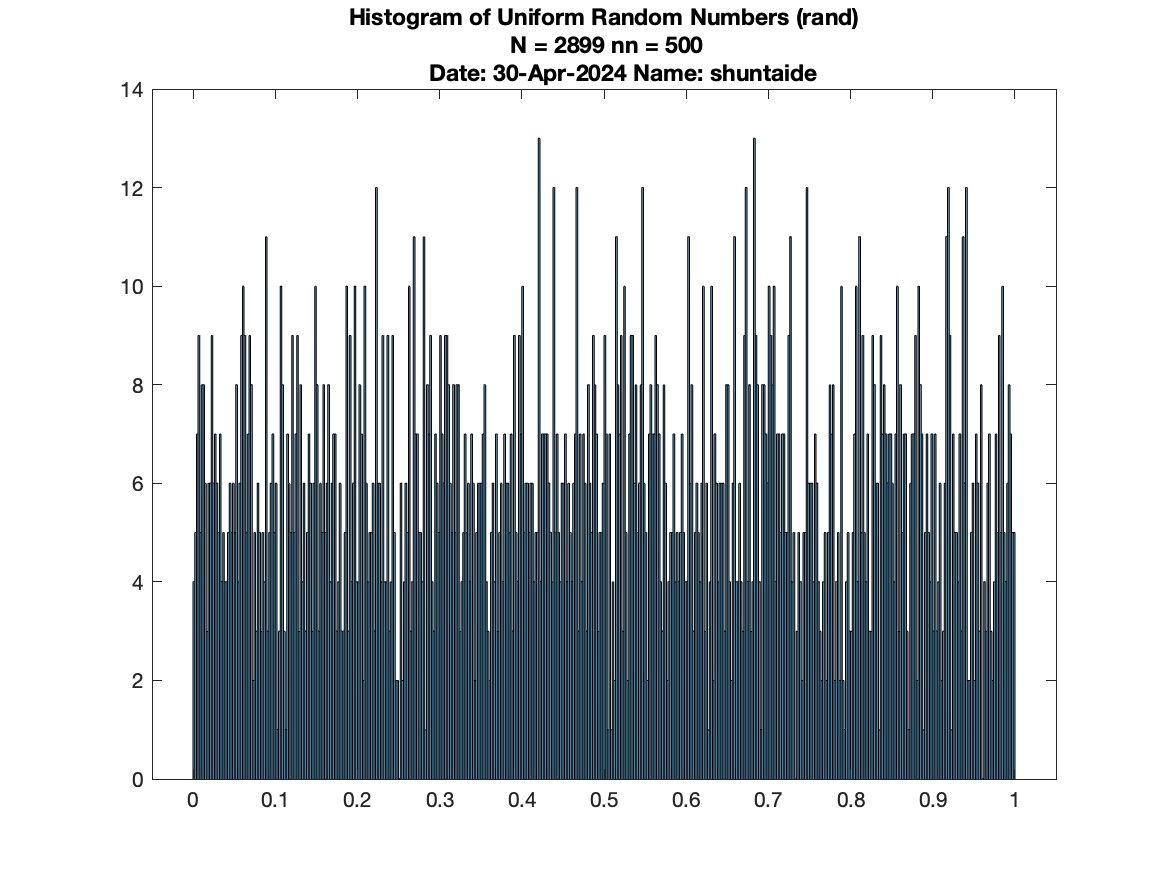
\includegraphics[width=0.8\textwidth]{src/figures/uniform/rand_hist_N=2899_nn=500.jpg}
		\subcaption{$N=2899$, $nn=500$}
	\end{subfigure}
	\begin{subfigure}{0.48\linewidth}
		\centering
		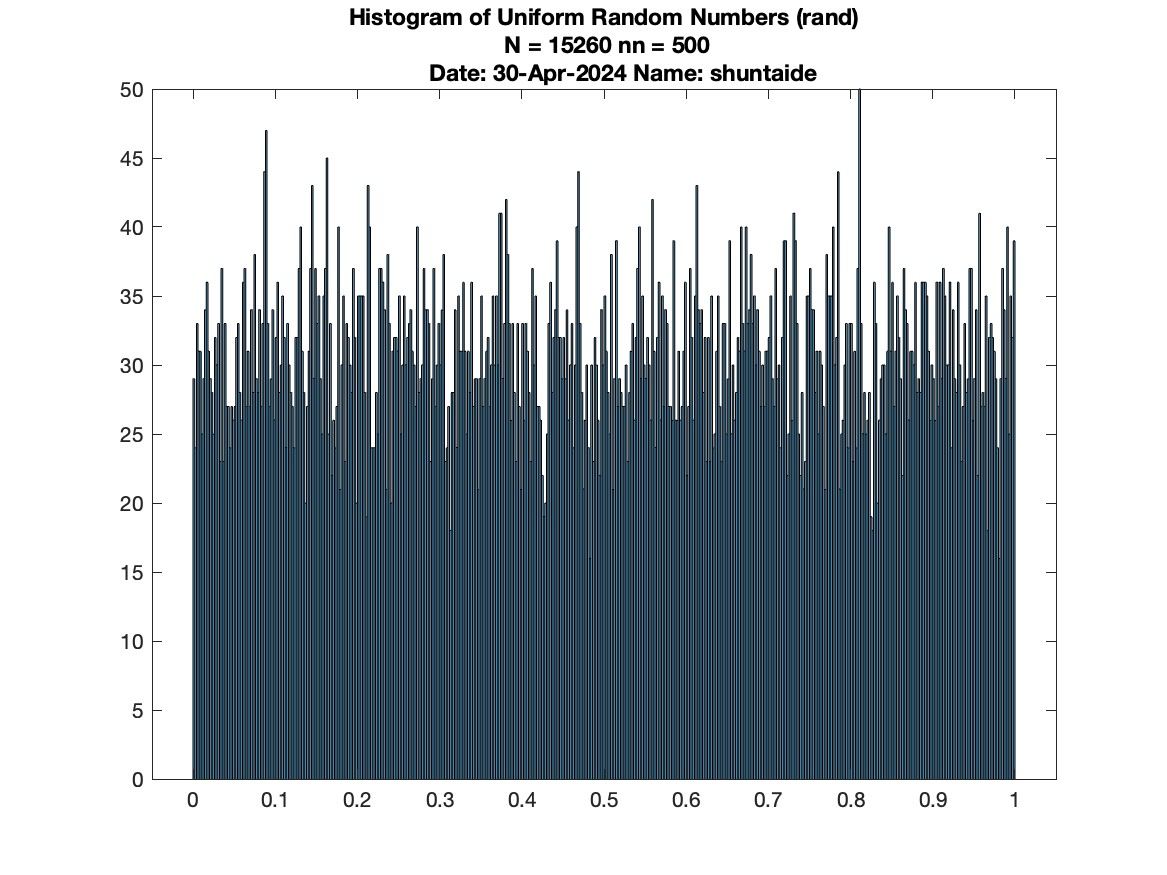
\includegraphics[width=0.8\textwidth]{src/figures/uniform/rand_hist_N=15260_nn=500.jpg}
		\subcaption{$N=15260$, $nn=500$}
	\end{subfigure}
	\begin{subfigure}{0.48\linewidth}
		\centering
		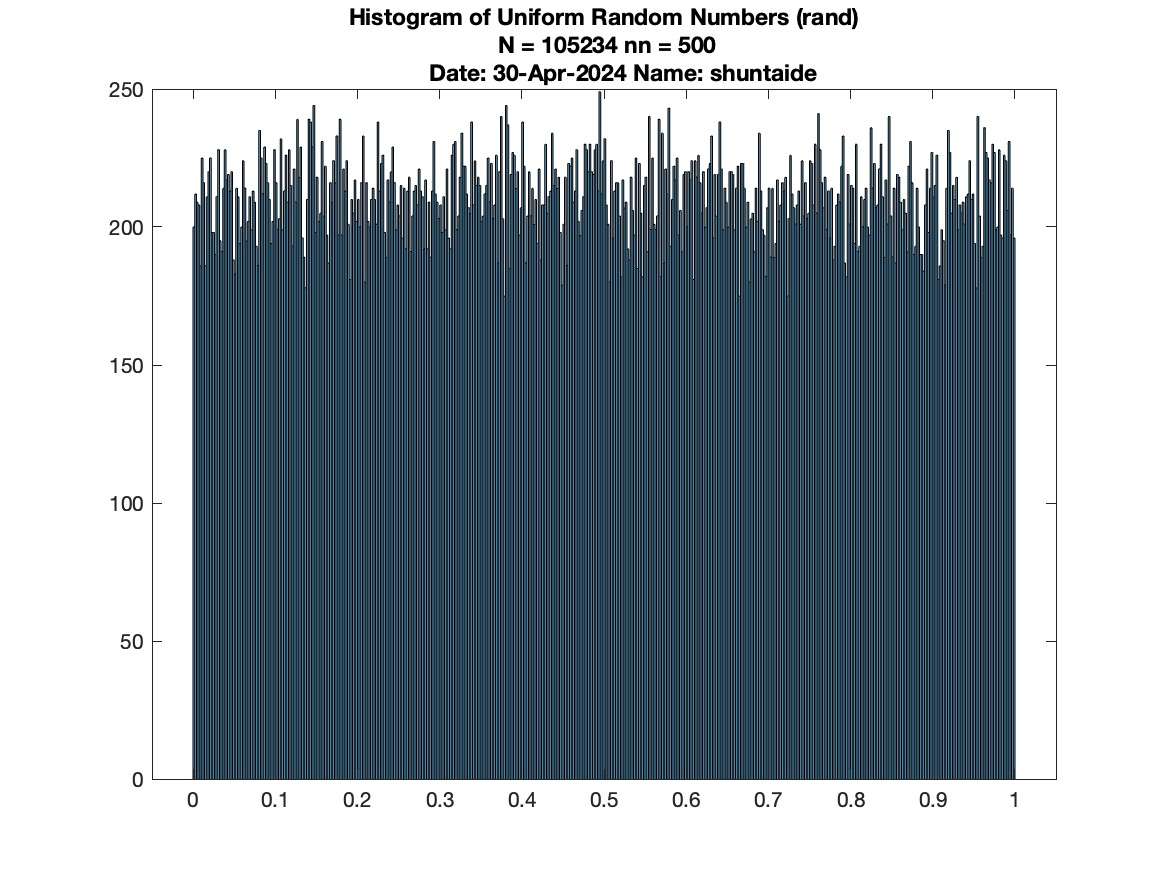
\includegraphics[width=0.8\textwidth]{src/figures/uniform/rand_hist_N=105234_nn=500.jpg}
		\subcaption{$N=105234$, $nn=500$}
	\end{subfigure}
	\begin{subfigure}{0.48\linewidth}
		\centering
		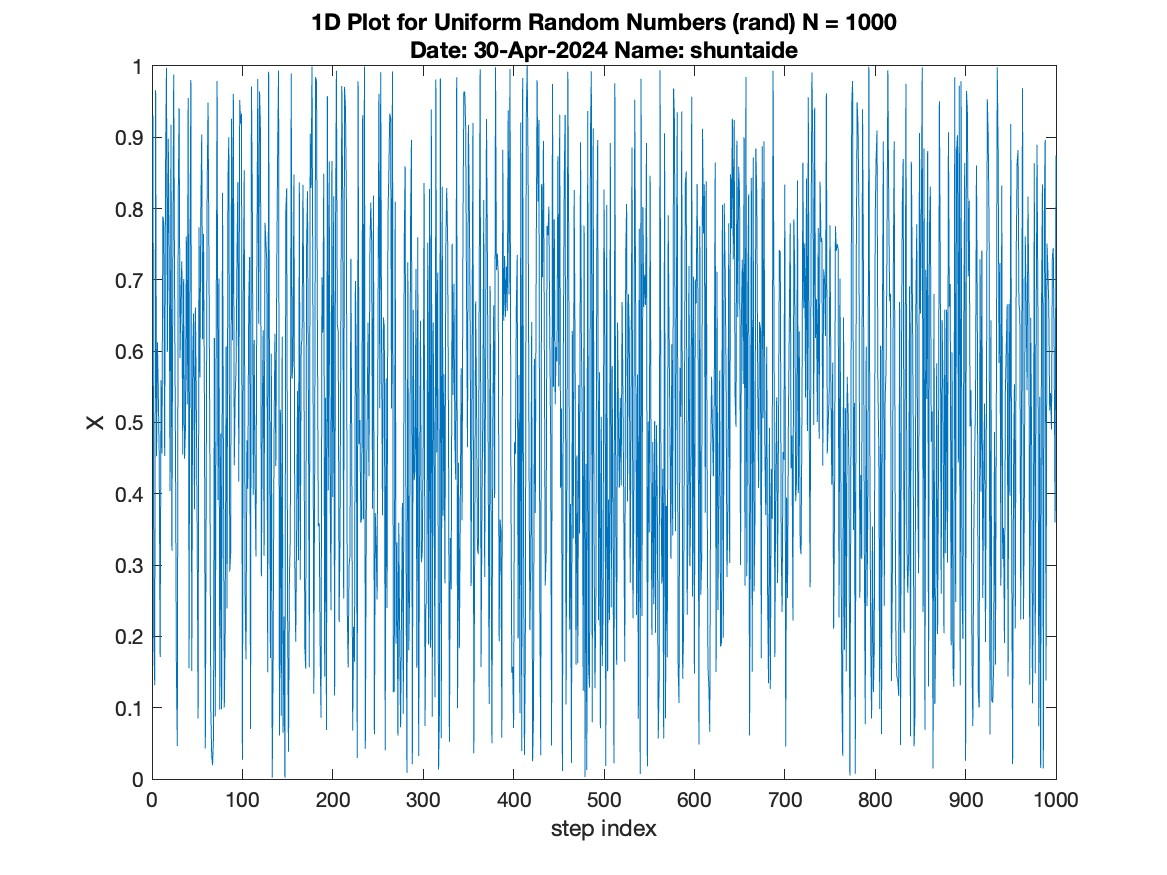
\includegraphics[width=0.8\textwidth]{src/figures/uniform/rand_1Dpl_N=1000.jpg}
		\subcaption{生成回と値の関係}\label{fig:uniform-1Dpl}
	\end{subfigure}
	\begin{subfigure}{0.48\linewidth}
		\centering
		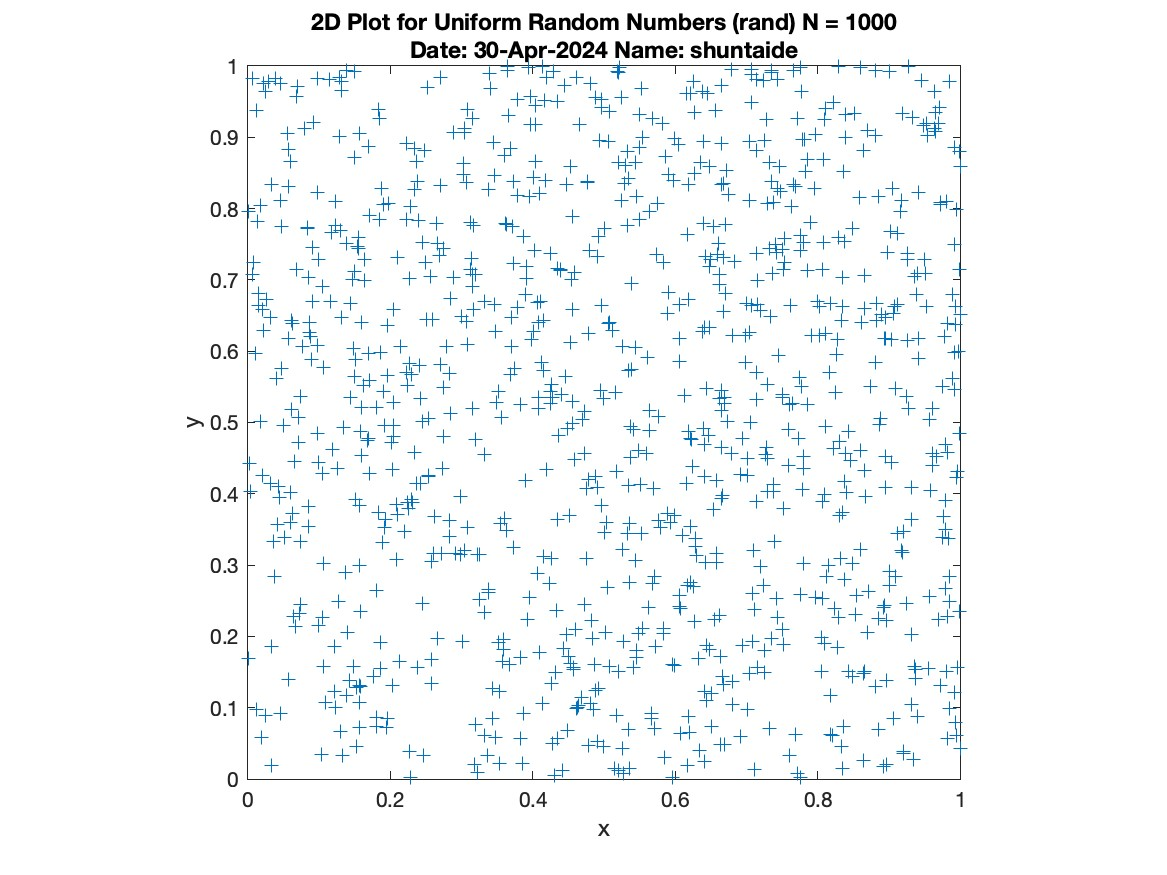
\includegraphics[width=0.8\textwidth]{src/figures/uniform/rand_2Dpl_N=1000.jpg}
		\subcaption{横軸が奇数回に生成された値、縦軸が偶数回に生成された値}\label{fig:uniform-2Dpl}
	\end{subfigure}
	\caption{一様乱数の生成結果}\label{fig:uniform-random}
\end{figure}
